% ============================================================================
% Chapitre 5 --- Scénario d'optimisation
% ============================================================================
\chapter{Scénario d'optimisation}
\label{chap:optimisation}

\begin{callout}
\textbf{Objectif~:} réduire le goulot d'étranglement au poste de contrôle qualité afin d'augmenter le débit global de la ligne de production.
\end{callout}

\section{Problème identifié}

Avec les paramètres initiaux (tableau~\ref{tab:parametres}), le contrôle qualité est le poste le plus lent~: 15~s par produit contre 8~s au traitement. Le jumeau numérique rend le phénomène visible sans calcul (figure~\ref{fig:vue_globale})~: au bout de quelques minutes, la file devant le contrôle atteint sa capacité de 8 produits, le traitement se bloque faute de place, puis l'alimentation à son tour. Le tableau de bord confirme le diagnostic~: le contrôle qualité est utilisé à 96~\% du temps, contre 53~\% pour le traitement et 35~\% pour l'alimentation, et un produit y attend en moyenne près de deux minutes.

\section{Solutions testées}

\begin{enumerate}
  \item \textbf{Contrôle automatisé}~: le temps de contrôle passe de 15 à 8~s grâce à une inspection automatisée. Cadence théorique~: $60/8 = 7{,}5$~produits/min, le traitement (8~s) devenant le nouveau poste limitant.
  \item \textbf{Deuxième poste de contrôle}~: deux machines de 15~s en parallèle, soit un temps effectif de 7{,}5~s. Cadence théorique~: 7{,}5~produits/min, limitée là aussi par le traitement.
  \item \textbf{Convoyeur adaptatif}~: le convoyeur ralentit devant une file chargée et la file maximale passe de 8 à 3 produits. Le débit théorique ne change pas (4~produits/min)~: cette solution vise l'accumulation, pas la cadence.
\end{enumerate}

\section{Protocole de comparaison}

Comparer deux scénarios en regardant l'animation n'est pas fiable~: une panne tombée au mauvais moment dans l'un des deux suffit à inverser la conclusion. Chaque scénario est donc simulé \textbf{pendant une heure}, sans affichage, avec la \textbf{même graine aléatoire} et les mêmes paramètres de fiabilité, de transfert et de rejet. Le bouton \enquote{Lancer la comparaison} du tableau de bord exécute exactement ce protocole (fonction \code{compare\_presets})~; les chiffres ci-dessous en sont la sortie brute, conservée dans \code{docs/\allowbreak rapport/\allowbreak data/\allowbreak resultats.json}.

\section{Résultats}

\begin{table}[H]
\centering
\caption{Comparaison avant / après sur 1~h simulée, pannes activées (graine 7).}
\label{tab:resultats}
\small
\begin{tabularx}{\textwidth}{@{}X cccc@{}}
\toprule
\textbf{Indicateur} & \textbf{Initiale} & \textbf{Contrôle 8~s} & \textbf{2 contrôles} & \textbf{Adaptatif} \\
\midrule
Produits finis / h & 218 & \textbf{390} (+79~\%) & 389 (+78~\%) & 218 (0~\%) \\
Cadence moyenne (/min) & 3,63 & \textbf{6,50} & 6,48 & 3,63 \\
Cadence théorique (/min) & 4,0 & 7,5 & 7,5 & 4,0 \\
Attente au contrôle (s) & 115 & \textbf{9} ($-$92~\%) & 16 ($-$86~\%) & 41 ($-$65~\%) \\
En-cours moyen (produits) & 19,0 & 13,4 ($-$30~\%) & 14,9 ($-$22~\%) & \textbf{9,4} ($-$51~\%) \\
Temps de séjour moyen (s) & 286 & \textbf{113} ($-$60~\%) & 129 ($-$55~\%) & 145 ($-$49~\%) \\
Rejets & 12 & 23 & 23 & 12 \\
Pannes / arrêts cumulés (s) & 25 / 589 & 28 / 635 & 29 / 712 & 25 / 589 \\
Goulot observé & Contrôle & Traitement & Traitement & Contrôle \\
\bottomrule
\end{tabularx}
\end{table}

\begin{figure}[H]
\centering
\begin{tikzpicture}
\begin{axis}[
  ybar, bar width=16pt, width=0.95\textwidth, height=6.2cm,
  ylabel={Produits finis par heure}, ymin=0, ymax=470,
  symbolic x coords={Initiale, Contrôle 8 s, 2 contrôles, Adaptatif},
  xtick=data, nodes near coords, nodes near coords style={font=\footnotesize},
  enlarge x limits=0.18, legend style={at={(0.5,1.03)}, anchor=south, legend columns=2, font=\footnotesize, draw=none},
  ymajorgrids, grid style={gray!20}, axis line style={gray!60}, tick label style={font=\footnotesize}
]
\addplot[fill=ensambleu, draw=ensambleu] coordinates {(Initiale,218) (Contrôle 8 s,390) (2 contrôles,389) (Adaptatif,218)};
\addplot[fill=ensambleu!35, draw=ensambleu!35] coordinates {(Initiale,226) (Contrôle 8 s,422) (2 contrôles,421) (Adaptatif,226)};
\legend{Avec pannes, Sans pannes}
\end{axis}
\end{tikzpicture}
\caption{Production horaire par scénario, avec et sans pannes.}
\label{fig:production}
\end{figure}

\begin{figure}[H]
\centering
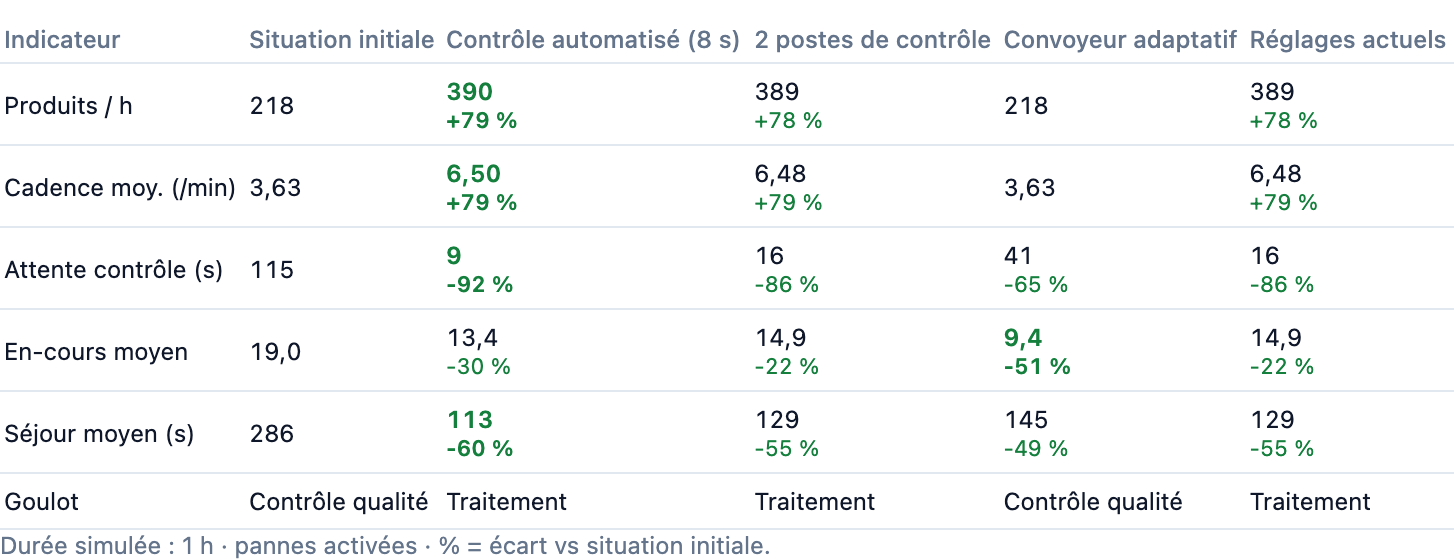
\includegraphics[width=\textwidth]{images/screenshots/comparaison.png}
\caption{Le même tableau dans l'interface (bouton \enquote{Lancer la comparaison})~; la colonne \enquote{Réglages actuels} reprend la configuration en cours.}
\label{fig:cmp_ui}
\end{figure}

\section{Analyse}

\paragraph{Le goulot se déplace.} Les deux premières solutions augmentent la production d'environ 79~\%, et le goulot passe du contrôle au traitement, comme prévu par le calcul théorique~: le traitement est désormais utilisé à 94~\% du temps. Toute amélioration supplémentaire devra donc porter sur le traitement. C'est le principe central de la théorie des contraintes~: optimiser un poste qui n'est pas le goulot ne sert à rien, et optimiser le goulot en fait apparaître un autre.

\paragraph{Contrôle automatisé ou deuxième poste~?} À débit égal, le contrôle automatisé est légèrement meilleur sur l'attente (9~s contre 16~s) et sur le temps de séjour, parce qu'un produit traverse le contrôle en 8~s au lieu de 15. Sur une ligne réelle, le deuxième poste apporterait en plus une redondance~: si l'une des deux machines tombe en panne, l'autre continue à 4~produits/min. Notre modèle ne capture pas cet avantage, car il traite la panne au niveau du poste entier (les deux machines s'arrêtent ensemble)~; c'est l'une des améliorations listées en perspective. Le choix entre les deux dépend donc d'informations que la simulation ne contient pas~: coût de l'automatisation, coût d'un poste et d'un opérateur supplémentaires, criticité des arrêts.

\paragraph{Le convoyeur adaptatif ne produit pas plus.} Il réduit l'en-cours de moitié et l'attente des deux tiers, sans perte de débit~; mais il ne déplace pas le goulot. Il a du sens en complément d'une des deux premières solutions (moins de stock entre postes, moins de produits immobilisés), pas à leur place.

\paragraph{Écart entre théorie et simulation.} L'énoncé estimait 240 produits/h avant et 450 après. La simulation donne 218 et 390. Sans pannes, la ligne initiale produit 226 produits finis \textbf{et} 12 rejetés, soit 238 produits sortis du contrôle~: l'écart restant avec 240 correspond au temps de démarrage (le premier produit n'atteint le contrôle qu'après 17~s, et le premier produit fini ne sort qu'après 41~s). Les pannes coûtent ensuite environ 4~\% de production sur la ligne initiale et 8~\% après optimisation~: une ligne plus rapide perd davantage de produits pour une même minute d'arrêt. Enfin, l'objectif de 450 produits/h n'est pas atteint, même sans pannes (422 finis + 24 rejets = 446 sorties)~: les 5~\% de rejets et le démarrage suffisent à l'expliquer. Le jumeau numérique a donc corrigé l'estimation initiale à la baisse de 13~\%, ce qui est précisément son rôle avant un investissement réel.

\begin{warn}
\textbf{Limite de la comparaison.} La graine aléatoire est identique pour tous les scénarios, mais les tirages divergent dès que la séquence d'événements diffère (un produit de plus contrôlé consomme un tirage de rejet de plus). Les pannes ne tombent donc pas exactement aux mêmes instants d'un scénario à l'autre. Pour des conclusions plus solides, il faudrait répéter la comparaison sur plusieurs graines et présenter des intervalles de confiance~; avec des écarts de l'ordre de 80~\%, la conclusion principale ne fait cependant pas de doute.
\end{warn}

\section{Démonstration dans le jumeau numérique}

\begin{enumerate}
  \item \textbf{Avant optimisation}~: lancer la situation initiale à vitesse $\times$10~; observer l'accumulation devant le contrôle, le blocage de l'amont et l'attente affichée (environ deux minutes).
  \item \textbf{Incident}~: provoquer une panne sur le traitement~; le voyant passe au rouge et la cadence chute.
  \item \textbf{Après optimisation}~: appliquer le contrôle automatisé à 8~s ou le deuxième poste~; la file se résorbe en quelques minutes et le goulot affiché passe au traitement.
  \item \textbf{Comparaison}~: lancer la comparaison, puis consulter et exporter les deux exécutions dans l'onglet Historique.
\end{enumerate}
